\documentclass{uofa-eng-assignment}
\usepackage{pythonhighlight}
\usepackage{amsmath}
\usepackage{enumerate}% http://ctan.org/pkg/enumerate
\usepackage{lipsum}
\usepackage{hyperref}
\usepackage{amsmath, amsthm, amssymb, amsfonts, physics}
\usepackage{mathtools}
\usepackage{graphicx}
\usepackage{fdsymbol}

\hypersetup{
    colorlinks=true,
    linkcolor=blue,
    filecolor=magenta,
    urlcolor=cyan,
    pdftitle={Overleaf Example},
    pdfpagemode=FullScreen,
}

\graphicspath{ {./images/} }

\DeclareRobustCommand{\rchi}{{\mathpalette\irchi\relax}}
\newcommand{\infdiv}{D\infdivx}
\newcommand{\irchi}[2]{\raisebox{\depth}{$#1\chi$}} % inner command, used by \rchi
\newcommand\aug{\fboxsep=-\fboxrule\!\!\!\fbox{\strut}\!\!\!}
\newcommand*{\name}{\textbf{Luke Nguyen}}
\newcommand*{\id}{\textbf{D5850A}}
\newcommand*{\course}{Statistical Methods and Data Analysis (EN.625.603)}
\newcommand*{\assignment}{Project 1}

\begin{document} \maketitle
%%%%%%%%%%%%%%%%%%%%%%%%%%%%%%%%%%%%%%%%%%%%%%%%%%%%%%%%%%%%%%%%%%%%%%%%%%%%%%%%%%%%%%%%%%%%%%%%%%%%    
\begin{enumerate}
    %%%%%%%%%%%%%%%%%%%%%%%%%%%%%%%%%%%%%%%%%%%%%%%%%%%%%%%%%%%%%%%%%%%%%%%%%%%%%%%%%%%%%%%%%%%%%%%%%%%%    
    %%%%%%%%%%%%%%%%%%%%%%%%%%%%%%%%%%%%%%%%%%%%%%%%%%%%%%%%%%%%%%%%%%%%%%%%%%%%%%%%%%%%%%%%%%%%%%%%%%%%    
    %%%%%%%%%%%%%%%%%%%%%%%%%%%%%%%%%%%%%%%%%%%%%%%%%%%%%%%%%%%%%%%%%%%%%%%%%%%%%%%%%%%%%%%%%%%%%%%%%%%%    
    %%%%%%%%%%%%%%%%%%%%%%%%%%%%%%%%%%%%%%%%%%%%%%%%%%%%%%%%%%%%%%%%%%%%%%%%%%%%%%%%%%%%%%%%%%%%%%%%%%%%    
    %%%%%%%%%%%%%%%%%%%%%%%%%%%%%%%%%%%%%%%%%%%%%%%%%%%%%%%%%%%%%%%%%%%%%%%%%%%%%%%%%%%%%%%%%%%%%%%%%%%%    
    \item[]
        \textbf{Project 1} \\
        Lead is toxic, particularly for young children, and for this reason government regulations
        severely restrict the amount of lead in our environment. But this was not always the
        case. In the early part of the 20th century, the underground water pipes in many US
        cities contained lead, and lead from these pipes leached into drinking water. In this
        exercise you will investigate the effect of these lead water pipes on infant mortality.
        \begin{enumerate}
            \item[(a)] Compute the average infant mortality rate $(Inf)$ for cities with lead pipes and for
                cities with non-lead pipes. Is there a statistically significant difference in the averages
            \item[(b)] The amount of lead leached from lead pipes depends on the chemistry of the
                water running through the pipes. The more acidic the water (that is, the lower
                the pH), the more lead is leached. Run a regression of $Inf$ on $Lead, pH$, and the
                interaction term $Lead \times pH$.
                \begin{enumerate}
                    \item The regression includes four coefficients (the intercept and the three
                          coefficients multiplying the regressors). Explain what each coefficient
                          measures.
                    \item Plot the estimated regression function relating $Inf$ to $pH$ for $Lead = 0$
                          and $Lead = 1$. Describe the differences in the regression functions and relate
                          these differences to the coefficients discussed in (i).
                    \item Does $Lead$ have a statistically significant effect on infant mortality?
                          Explain.
                    \item Does the effect of $Lead$ on infant mortality depend on $pH$? Is this
                          dependence statistically significant?
                    \item What is the average value of $pH$ in the sample? At this $pH$ level, what is
                          the estimated effect of $Lead$ on infant mortality? What is the standard
                          deviation of $pH$? Suppose that the $pH$ level is on standard deviation lower
                          than the average level of $pH$ in the sample; what is the estimated effect of
                          $Lead$ on infant mortality? What if $pH$ is one standard deviation higher than
                          the average value?
                    \item Construct a $95\%$ confidence interval for the effect of Lead on infant
                          mortality when $pH = 6.5$.

                \end{enumerate}
            \item[(c)] The analysis in (b) may suffer from omitted variable bias because it neglects
                factors that affect infant mortality and that might potentially be correlated with
                $Lead$ and $pH$. Investigate this concern, using the other variables in the data set. \\
        \end{enumerate}

        \textbf{Solution}
        \begin{enumerate}
            \item[(a)]
                Using Python with Pandas library, we have the following statistics with
                $n, \bar{x}, s_x$ for lead and $m, \bar{y}, s_y$ for non-lead.
                \begin{align*}
                    n & = 55 \quad \bar{x} = 0.3812 \quad s_x = 0.1478  \\
                    m & = 117 \quad \bar{y} = 0.4033 \quad s_y = 0.1531
                \end{align*}
                Test hypothesis is as follows:
                \begin{align*}
                    \text{H}_0: \mu_{x} & = \mu_{y} \\
                    \text{H}_1: \mu_{x} & < \mu_{y}
                \end{align*}
                The level of significance is $\alpha = 0.05$. \\
                The degrees of freedom and critical value are as follows:
                \begin{align*}
                    df             & = n + m - 2     \\
                                   & = 55 + 117 - 2  \\
                                   & = 170           \\
                    t_{\alpha, df} & = t_{0.05, 170} \\
                                   & = 1.6539        \\
                \end{align*}
                The pooled standard deviation is as follows:
                \begin{align*}
                    s_p & = \sqrt{\frac{(n - 1)s_x^2 + (m - 1)s_y^2}{n + m - 2}}    \\
                        & = \sqrt{\frac{(55 - 1)0.1478^2 + (117 - 1)0.1531^2}{170}} \\
                        & = 0.1514
                \end{align*}
                The test statistic is as follows:
                \begin{align*}
                    t & = \frac{\bar{x} - \bar{y}}{s_p\sqrt{\frac{1}{n} + \frac{1}{m}}}     \\
                      & = \frac{0.3812 - 0.4033}{0.1514\sqrt{\frac{1}{55} + \frac{1}{117}}} \\
                      & = -0.8923
                \end{align*}
                Because $t = -0.8923 > -t_{\alpha, df} = -1.6539$, we fail to reject the null hypothesis.
            \item[(b)]
                \begin{enumerate}
                    \item The coefficients were calculated using Python and Pandas are as follows
                          \begin{figure}[h]
                              \centering
                              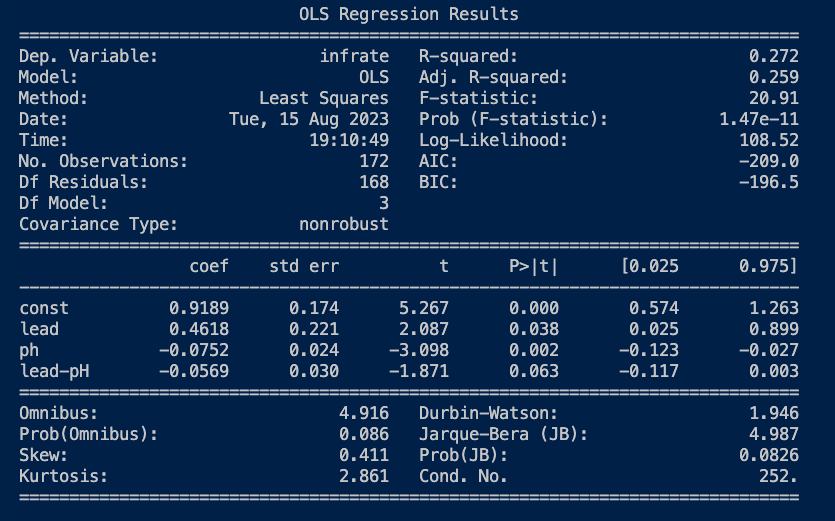
\includegraphics[width=0.45\textwidth]{p1-b-i.png}
                          \end{figure} \\
                          The regression includes four coefficients (the intercept and the three
                          coefficients multiplying the regressors).
                          \begin{align*}
                              \text{Inf} & = \beta_0 + \beta_1\text{Lead} + \beta_2\text{pH} + \beta_3\text{Lead}\times\text{pH} \\
                          \end{align*}

                          \begin{align*}
                              \beta_0 & = 0.9189  \\
                              \beta_1 & = 0.4618  \\
                              \beta_2 & = -0.0752 \\
                              \beta_3 & = -0.0569
                          \end{align*}
                          $\beta_0 = 0.9189$ is the average infant mortality when $Lead = 0$ and $pH = 0$. \\
                          $\beta_1 = 0.4618$ is the effect of $Lead$ on infant mortality when $pH = 0$. \\
                          $\beta_2 = -0.0752$ is the effect of $pH$ on infant mortality when $Lead = 0$. \\
                          $\beta_3 = -0.0569$ is the effect of $pH$ on infant mortality when $Lead = 1$. \\

                    \item The estimated regression function relating $Inf$ to $pH$ for $Lead = 0$ is as
                          follows
                          \begin{align*}
                              \text{Inf} & = \beta_0 + \beta_2\text{pH} + \epsilon \\
                                         & = 0.9189 - 0.0752\text{pH} + \epsilon
                          \end{align*}
                          The estimated regression function relating $Inf$ to $pH$ for $Lead = 1$ is as follows
                          \begin{align*}
                              \text{Inf} & = \beta_0 + \beta_1 + \beta_2\text{pH} + \beta_3\text{pH} + \epsilon \\
                                         & = 0.9189 + 0.4618 - 0.0752\text{pH} - 0.0569\text{pH} + \epsilon     \\
                                         & = 1.3807 - 0.1321\text{pH} + \epsilon
                          \end{align*}
                          \begin{figure}[h]
                              \centering
                              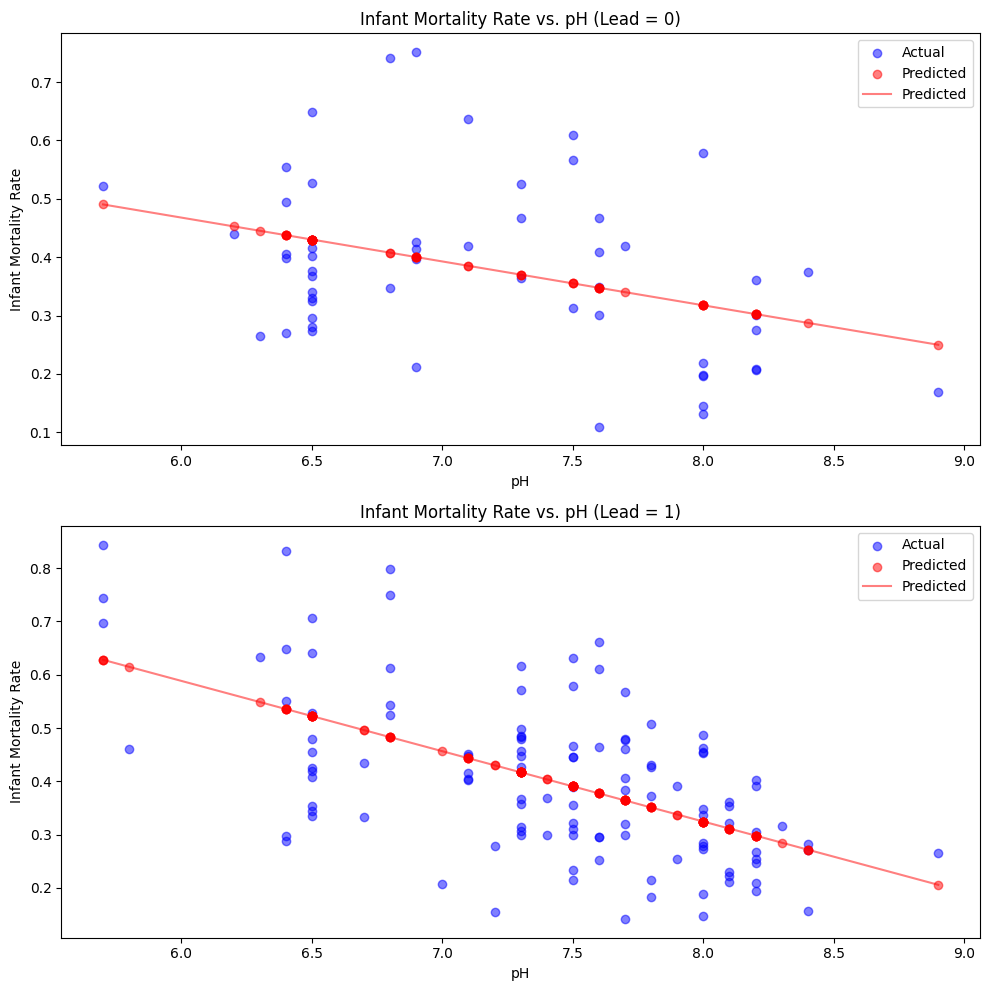
\includegraphics[width=0.68\textwidth]{p1-b-ii.png}
                          \end{figure} \\
                    \item To determine if Lead has a statistically significant effect on infant
                          mortality, we use $F-$ test from Python as follows
                          \begin{figure}[h]
                              \centering
                              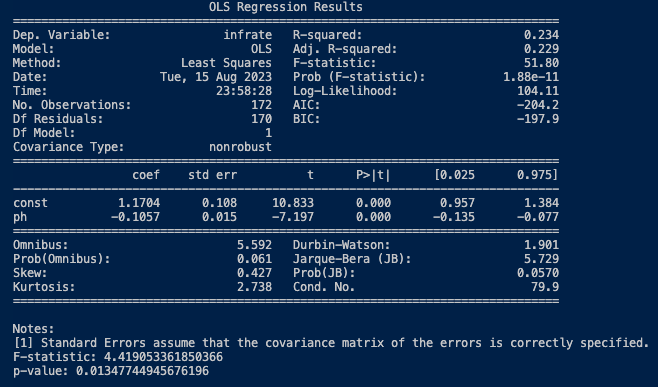
\includegraphics[width=0.68\textwidth]{p1-b-iii.png}
                          \end{figure} \\
                          We have the following statistics
                          \begin{align*}
                              F       & = 4.4191 \\
                              p-value & = 0.0134
                          \end{align*}
                          Thus, we can conclude that Lead has a statistically significant effect on infant mortality.
                    \item $p-value$ of the interaction $lead \times pH$ is $0.0631$ which is greater than
                          $\alpha = 0.05$. Thus, we can conclude that the effect of $Lead$ on infant mortality does
                          not depend on $pH$.
                          \begin{figure}[h]
                              \centering
                              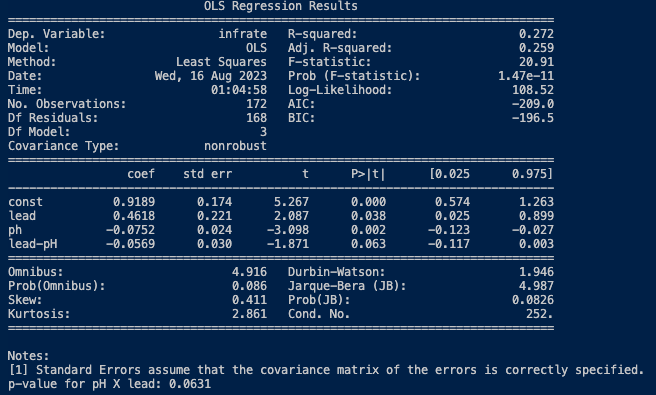
\includegraphics[width=0.68\textwidth]{p1-b-iv.png}
                          \end{figure} \\
                    \item We have mean and standard deviation of $pH$ as follows
                          \begin{figure}[h]
                              \centering
                              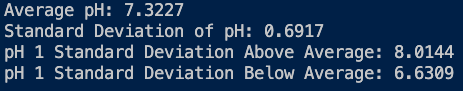
\includegraphics[width=0.68\textwidth]{p1-b-v.png}
                          \end{figure} \\
                          \begin{align*}
                              \bar{pH} & = 7.3227 \\
                              s_{pH}   & = 0.6917
                          \end{align*}
                          The estimated regression function relating $Inf$ to $pH$ for $Lead = 0$ is as
                          follows
                          \begin{align*}
                              \text{Inf} & = \beta_0 + \beta_2\text{pH} \\
                                         & = 0.9189 - 0.0752(7.3227)    \\
                                         & = 0.3682
                          \end{align*}
                          The estimated regression function relating $Inf$ to $pH$ for $Lead = 1$ is
                          as follows
                          \begin{align*}
                              \text{Inf} & = \beta_0 + \beta_1 + \beta_2\text{pH} + \beta_3\text{pH} \\
                                         & = 0.9189 + 0.4618 - 0.0752(7.3227) - 0.0569(7.3227)       \\
                                         & = 0.4134
                          \end{align*}
                          Thus, the difference in the estimated infant mortality rates for $Lead = 0$ and $Lead = 1$ is
                          \begin{align*}
                              \text{Inf}_{Lead = 0} - \text{Inf}_{Lead = 1} & = 0.3682 - 0.4134 \\
                                                                            & = -0.0452
                          \end{align*}
                          $pH$ one standard deviation above its mean is $7.3227 + 0.6917 = 8.0144$.
                          The estimated regression function relating $Inf$ to $pH$ for $Lead = 0$ is as
                          follows
                          \begin{align*}
                              \text{Inf} & = \beta_0 + \beta_2\text{pH} \\
                                         & = 0.9189 - 0.0752(8.0144)    \\
                                         & = 0.3162
                          \end{align*}
                          The estimated regression function relating $Inf$ to $pH$ for $Lead = 1$ is
                          as follows
                          \begin{align*}
                              \text{Inf} & = \beta_0 + \beta_1 + \beta_2\text{pH} + \beta_3\text{pH} \\
                                         & = 0.9189 + 0.4618 - 0.0752(8.0144) - 0.0569(8.0144)       \\
                                         & = 0.3220
                          \end{align*}
                          Thus, the difference in the estimated infant mortality rates for $Lead = 0$ and $Lead = 1$ is
                          \begin{align*}
                              \text{Inf}_{Lead = 0} - \text{Inf}_{Lead = 1} & = 0.3162 - 0.3220 \\
                                                                            & = -0.0058
                          \end{align*}
                          $pH$ one standard deviation below its mean is $7.3227 - 0.6917 = 6.6310$.
                          The estimated regression function relating $Inf$ to $pH$ for $Lead = 0$ is as
                          follows
                          \begin{align*}
                              \text{Inf} & = \beta_0 + \beta_2\text{pH} \\
                                         & = 0.9189 - 0.0752(6.6310)    \\
                                         & = 0.4202
                          \end{align*}
                          The estimated regression function relating $Inf$ to $pH$ for $Lead = 1$ is
                          as follows
                          \begin{align*}
                              \text{Inf} & = \beta_0 + \beta_1 + \beta_2\text{pH} + \beta_3\text{pH} \\
                                         & = 0.9189 + 0.4618 - 0.0752(6.6310) - 0.0569(6.6310)       \\
                                         & = 0.5047
                          \end{align*}
                          Thus, the difference in the estimated infant mortality rates for $Lead = 0$ and $Lead = 1$ is
                          \begin{align*}
                              \text{Inf}_{Lead = 0} - \text{Inf}_{Lead = 1} & = 0.4202 - 0.5047 \\
                                                                            & = -0.0844
                          \end{align*}
                    \item
                          The standard error of the estimated infant mortality rate is
                          \begin{align*}
                              s_{\text{Inf}} & = 0.1513
                          \end{align*}
                          The estimated mortality rate for $Lead = 0$ and $pH = 6.5$ is
                          \begin{align*}
                              \text{Inf} & = \beta_0 + \beta_2\text{pH} \\
                                         & = 0.9189 - 0.0752(6.5)       \\
                                         & = 0.4301
                          \end{align*}
                          The estimated mortality rate for $Lead = 1$ and $pH = 6.5$ is
                          \begin{align*}
                              \text{Inf} & = \beta_0 + \beta_1 + \beta_2\text{pH} + \beta_3\text{pH} \\
                                         & = 0.9189 + 0.4618 - 0.0752(6.5) - 0.0569(6.5)             \\
                                         & = 0.5221
                          \end{align*}
                          Degrees of freedom and t-critical value for $\alpha = 0.05$ are as follows
                          \begin{align*}
                              n - p - 1          & = 172 - 3 - 1    \\
                                                 & = 168            \\
                              t_{\alpha / 2, df} & = t_{0.025, 168} \\
                                                 & = 2.262
                          \end{align*}
                          The $95\%$ confidence interval for the difference in the estimated infant mortality rates for $Lead = 0$ and $Lead = 1$ is
                          \begin{align*}
                               & = \text{Inf}_{Lead = 0} - \text{Inf}_{Lead = 1} \pm t_{\alpha / 2, df}s_{\text{Inf}}\sqrt{\frac{1}{n_0} + \frac{1}{n_1}} \\
                               & = -0.0920 \pm 2.262(0.1513)\sqrt{\frac{1}{55} + \frac{1}{117}}                                                           \\
                               & = (-0.1480, -0.0360)
                          \end{align*}
                \end{enumerate}
            \item[(c)] Of the 15 columns in the dataset, the analysis obmitted the majority of other variables
                which might have an effect on infant mortality and correlated with $Lead$ and $pH$.
                \begin{enumerate}
                    \item We can investigate water hardness index. \\ After adding $Hardness$ to the
                          model, and we can see that its $p$-value is $0.924$, which is greater than
                          $0.05$. Thus, we can conclude that $Hardness$ is not statistically significant
                          in the model.
                    \item We can investigate mom age index. \\ After adding $Age$ to the model, and we
                          can see that its $p$-value is $0.416$, which is greater than $0.05$. Thus, we
                          can conclude that $Age$ is not statistically significant in the model.
                \end{enumerate}
                \begin{figure}[h]
                    \centering
                    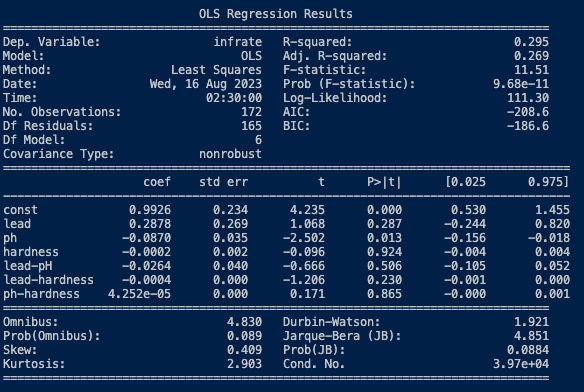
\includegraphics[width=0.68\textwidth]{p1-c-i.png}
                \end{figure}
                \begin{figure}[h]
                    \centering
                    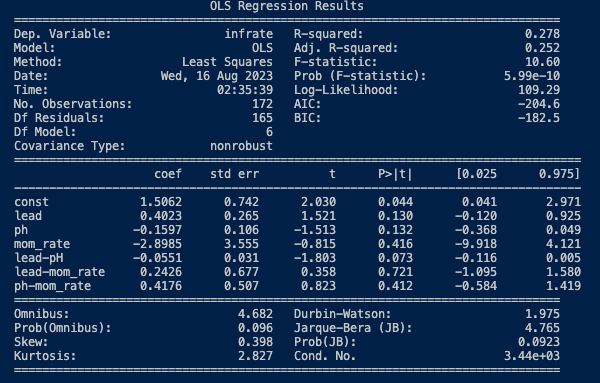
\includegraphics[width=0.68\textwidth]{p1-c-ii.png}
                \end{figure} \clearpage
        \end{enumerate}
\end{enumerate}
\begin{python}
# All code used to generate the results are shown below
import pandas as pd
import numpy as np
import statsmodels.api as sm
from scipy import stats
import scipy.stats
import matplotlib.pyplot as plt


class LeadMortalityDataframe:

    df = None

    column_name_year = None
    column_name_city = None
    column_name_state = None
    column_name_age = None
    column_name_hardness = None
    column_name_ph = None
    column_name_infrate = None
    column_name_typhoid_rate = None
    column_name_np_tub_rate = None
    column_name_mom_rate = None
    column_name_population = None
    column_name_precipitation = None
    column_name_temperature = None
    column_name_lead = None
    column_name_foreign_share = None

    def __init__(self):
        file_path = 'lead_mortality.xlsx'
        file_sheet_name = 'Data'

        self.df = pd.read_excel(file_path, sheet_name=file_sheet_name)
        self.column_name_year = self.df.columns[0]
        self.column_name_city = self.df.columns[1]
        self.column_name_state = self.df.columns[2]
        self.column_name_age = self.df.columns[3]
        self.column_name_hardness = self.df.columns[4]
        self.column_name_ph = self.df.columns[5]
        self.column_name_infrate = self.df.columns[6]
        self.column_name_typhoid_rate = self.df.columns[7]
        self.column_name_np_tub_rate = self.df.columns[8]
        self.column_name_mom_rate = self.df.columns[9]
        self.column_name_population = self.df.columns[10]
        self.column_name_precipitation = self.df.columns[11]
        self.column_name_temperature = self.df.columns[12]
        self.column_name_lead = self.df.columns[13]
        self.column_name_foreign_share = self.df.columns[14]

    def log_dataframe_info(self):
        print(f'Number of rows: {self.df.shape[0]}')
        print(f'Number of columns: {self.df.shape[1]}')
        print('Column names:')
        print(self.df.columns.tolist())
        print('Data summary:')
        print(self.df.describe(include='all'))

    def get_lead_by_condition(self, condition):
        return self.df[self.df[self.column_name_lead] == condition]

    def get_infrate_by_lead_condition(self, lead_condition):
        df = self.get_lead_by_condition(lead_condition)
        return df[self.column_name_infrate]


def part_a_solution():
    lead_mortality = LeadMortalityDataframe()

    infrate_lead_0 = lead_mortality.get_infrate_by_lead_condition(0)
    infrate_lead_1 = lead_mortality.get_infrate_by_lead_condition(1)

    n = infrate_lead_0.shape[0]
    m = infrate_lead_1.shape[0]
    avg_x = infrate_lead_0.mean()
    avg_y = infrate_lead_1.mean()
    std_x = infrate_lead_0.std()
    std_y = infrate_lead_1.std()
    level_of_significance = 0.05
    d_freedom = n + m - 2
    t_a_df = -scipy.stats.t.ppf(level_of_significance, d_freedom)
    std_pooled = np.sqrt(
        ((n - 1) * pow(std_x, 2) + (m - 1) * pow(std_y, 2)) / d_freedom)
    t_statistics = (avg_x - avg_y) / (std_pooled * np.sqrt(1/n + 1/m))
    print(f'n: {n}')
    print(f'm: {m}')
    print(f'avg_x: {avg_x:.4f}')
    print(f'avg_y: {avg_y:.4f}')
    print(f'std_x: {std_x:.4f}')
    print(f'std_y: {std_y:.4f}')
    print(f'std_pooled: {std_pooled:.4f}')
    print(f't_a_df: {t_a_df:.4f}')
    print(f't_statistics: {t_statistics:.4f}')


def part_b_i_solution():
    lead_mortality = LeadMortalityDataframe()
    lead_mortality.df["lead-pH"] = lead_mortality.df[lead_mortality.column_name_lead] * \
        lead_mortality.df[lead_mortality.column_name_ph]

    x = sm.add_constant(lead_mortality.df[[lead_mortality.column_name_lead,
                                           lead_mortality.column_name_ph, "lead-pH"]])
    y = lead_mortality.df[lead_mortality.column_name_infrate]
    model = sm.OLS(y, x)
    results = model.fit()
    print(results.summary())


def part_b_ii_solution():
    lead_mortality = LeadMortalityDataframe()
    lead_mortality.df["lead-pH"] = lead_mortality.df[lead_mortality.column_name_lead] * \
        lead_mortality.df[lead_mortality.column_name_ph]

    x = sm.add_constant(lead_mortality.df[[lead_mortality.column_name_lead,
                                           lead_mortality.column_name_ph, "lead-pH"]])
    y = lead_mortality.df[lead_mortality.column_name_infrate]
    model = sm.OLS(y, x)
    results = model.fit()
    fig, ax = plt.subplots(2, 1, figsize=(10, 10))

    lead_mortality.df['pred_infrate'] = results.predict(x)

    df_lead0 = lead_mortality.df[lead_mortality.df['lead'] == 0]
    ax[0].scatter(df_lead0['ph'], df_lead0['infrate'],
                  color='blue', alpha=0.5, label='Actual')
    sorted_df_lead0 = df_lead0.sort_values(by='ph')
    ax[0].plot(sorted_df_lead0['ph'], sorted_df_lead0['pred_infrate'],
               color='red', alpha=0.5, label='Predicted')
    ax[0].set_title('Infant Mortality Rate vs. pH (Lead = 0)')
    ax[0].set_xlabel('pH')
    ax[0].set_ylabel('Infant Mortality Rate')
    ax[0].legend()

    df_lead1 = lead_mortality.df[lead_mortality.df['lead'] == 1]
    ax[1].scatter(df_lead1['ph'], df_lead1['infrate'],
                  color='blue', alpha=0.5, label='Actual')
    sorted_df_lead1 = df_lead1.sort_values(by='ph')
    ax[1].plot(sorted_df_lead1['ph'], sorted_df_lead1['pred_infrate'],
               color='red', alpha=0.5, label='Predicted')
    ax[1].set_title('Infant Mortality Rate vs. pH (Lead = 1)')
    ax[1].set_xlabel('pH')
    ax[1].set_ylabel('Infant Mortality Rate')
    ax[1].legend()

    plt.tight_layout()
    plt.show()


def part_b_iii_solution():
    lead_mortality = LeadMortalityDataframe()
    lead_mortality.df["lead-pH"] = lead_mortality.df[lead_mortality.column_name_lead] * \
        lead_mortality.df[lead_mortality.column_name_ph]
    x = sm.add_constant(lead_mortality.df[[lead_mortality.column_name_lead,
                                           lead_mortality.column_name_ph, "lead-pH"]])
    y = lead_mortality.df[lead_mortality.column_name_infrate]
    results = sm.OLS(y, x).fit()

    x_ph = sm.add_constant(lead_mortality.df[[lead_mortality.column_name_ph]])
    results_ph = sm.OLS(y, x_ph).fit()

    f_test = results.compare_f_test(results_ph)
    print(results_ph.summary())
    print('F-statistic:', f_test[0])
    print('p-value:', f_test[1])


def part_b_iv_solution():
    lead_mortality = LeadMortalityDataframe()
    lead_mortality.df["lead-pH"] = lead_mortality.df[lead_mortality.column_name_lead] * \
        lead_mortality.df[lead_mortality.column_name_ph]
    x = sm.add_constant(lead_mortality.df[[lead_mortality.column_name_lead,
                                           lead_mortality.column_name_ph, "lead-pH"]])
    y = lead_mortality.df[lead_mortality.column_name_infrate]
    results = sm.OLS(y, x).fit()
    model = sm.OLS(y, x)
    results = model.fit()
    print(results.summary())
    p_values_pHxLead = results.pvalues["lead-pH"]
    print(f'p-value for pH X lead: {p_values_pHxLead:.4f}')


def part_b_v_solution():
    lead_mortality = LeadMortalityDataframe()
    avg_ph = lead_mortality.df[lead_mortality.column_name_ph].mean()
    std_ph = lead_mortality.df[lead_mortality.column_name_ph].std()
    ph_1_std_above = avg_ph + std_ph
    ph_1_std_below = avg_ph - std_ph
    print(f'Average pH: {avg_ph:.4f}')
    print(f'Standard Deviation of pH: {std_ph:.4f}')
    print(f'pH 1 Standard Deviation Above Average: {ph_1_std_above:.4f}')
    print(f'pH 1 Standard Deviation Below Average: {ph_1_std_below:.4f}')


def part_b_vi_solution():
    lead_mortality = LeadMortalityDataframe()
    std_infrate = lead_mortality.df[lead_mortality.column_name_infrate].std()

    print(f'Standard Deviation of Infant Mortality Rate: {std_infrate:.4f}')


def part_c_i_solution():
    lead_mortality = LeadMortalityDataframe()
    lead_mortality.df["lead-pH"] = lead_mortality.df[lead_mortality.column_name_lead] * \
        lead_mortality.df[lead_mortality.column_name_ph]
    lead_mortality.df["lead-hardness"] = lead_mortality.df[lead_mortality.column_name_lead] * \
        lead_mortality.df[lead_mortality.column_name_hardness]
    lead_mortality.df["ph-hardness"] = lead_mortality.df[lead_mortality.column_name_ph] * \
        lead_mortality.df[lead_mortality.column_name_hardness]

    x = sm.add_constant(lead_mortality.df[[lead_mortality.column_name_lead,
                                           lead_mortality.column_name_ph,
                                           lead_mortality.column_name_hardness,
                                           "lead-pH",
                                           "lead-hardness",
                                           "ph-hardness"]])
    y = lead_mortality.df[lead_mortality.column_name_infrate]
    model = sm.OLS(y, x)
    results = model.fit()
    print(results.summary())


def part_c_ii_solution():
    lead_mortality = LeadMortalityDataframe()
    lead_mortality.df["lead-pH"] = lead_mortality.df[lead_mortality.column_name_lead] * \
        lead_mortality.df[lead_mortality.column_name_ph]
    lead_mortality.df["lead-mom_rate"] = lead_mortality.df[lead_mortality.column_name_lead] * \
        lead_mortality.df[lead_mortality.column_name_mom_rate]
    lead_mortality.df["ph-mom_rate"] = lead_mortality.df[lead_mortality.column_name_ph] * \
        lead_mortality.df[lead_mortality.column_name_mom_rate]

    x = sm.add_constant(lead_mortality.df[[lead_mortality.column_name_lead,
                                           lead_mortality.column_name_ph,
                                           lead_mortality.column_name_mom_rate,
                                           "lead-pH",
                                           "lead-mom_rate",
                                           "ph-mom_rate"]])
    y = lead_mortality.df[lead_mortality.column_name_infrate]
    model = sm.OLS(y, x)
    results = model.fit()
    print(results.summary())


if __name__ == '__main__':
    part_c_ii_solution()

\end{python}
%%%%%%%%%%%%%%%%%%%%%%%%%%%%%%%%%%%%%%%%%%%%%%%%%%%%%%%%%%%%%%%%%%%%%%%%%%%%%%%%%%%%%%%%%%%%%%%%%%%%    
\end{document}